\chapter{Approach}

The \glstext{YAML} standard is extensive. The document describing the serialization language includes about 200 parameterized \gls{BNF} grammar rules~\cite{ben2009yaml}. To simplify the parser development we decided to first determine a useful subset of \glstext{YAML}. For this purpose we discussed the language with other Elektra developers. The first part of this chapter contains a review detailing this discussion.

In the second part we describe how we mapped Elektra’s two basic types, \cc{Key} and \cc{KeySet} to \glstext{YAML}.

\section{Discussion}

In the discussion 9 participants answered questions about the usefulness of certain \glstext{YAML} features for \href{https://www.libelektra.org}{Elektra}. We introduced the \glstext{YAML} syntax in a \href{https://github.com/sanssecours/YAML-Presentation/releases/download/v1.0/Presentation.pdf}{presentation}. After we talked about a certain part of YAML, we answered questions the participants had about the information presented so far. Afterwards we asked the participants to fill in parts of a \href{https://github.com/sanssecours/YAML-Presentation/blob/master/Questionnaire.md}{questionnaire} about the newly introduced feature set. The questionnaire consisted of checkboxes for each feature. A checked box indicates that the participant considers a feature useful for Elektra.

\subsection{Participants}

All of the participants were at least partially familiar with Elektra. Some also had previous experience with \glstext{YAML}. Seven of them listened to the presentation, while one participant was late and another one participated via email. The email participant received a copy of the presentation slides and the questionnaire.

\subsection{Results}

In the following bar charts the term “Yes” refers to a checked box for the specific feature. The term “?” means that the participant did not know enough about a part of \glstext{YAML} and therefore marked the checkbox for one feature, or the heading for multiple features, with a question mark. The value before the term “No” specifies the number of unchecked boxes minus the number of boxes marked with “?”.

\subsubsection{Scalars}

\paragraph{Flow Scalars}

\begin{figure}[H]
  \begin{minipage}[t]{0.48\textwidth}
    \vspace{0pt}
    \begin{bchart}[max=9, width=0.85\textwidth]
      \bcbar[text=3, value=Yes, color=orange]{3}
      \bcbar[text=6, value=No, color=Aqua]{6}
    \end{bchart}
  \end{minipage}
  \begin{minipage}[t]{0.48\textwidth}
    \vspace{0pt}
    \begin{yamlcode}
      Plain String
    \end{yamlcode}
  \end{minipage}
  \caption{Plain Flow Scalar}
\end{figure}

\begin{figure}[H]
  \begin{minipage}[t]{0.48\textwidth}
    \vspace{0pt}
    \begin{bchart}[max=9, width=0.85\textwidth]
      \bcbar[text=2, value=Yes, color=orange]{2}
      \bcbar[text=7, value=No, color=Aqua]{7}
    \end{bchart}
  \end{minipage}
  \begin{minipage}[t]{0.48\textwidth}
    \vspace{0pt}
    \begin{yamlcode}
      'Single Quoted ''String'''
    \end{yamlcode}
  \end{minipage}
  \caption{Single Quoted Flow Scalar}
\end{figure}

\begin{figure}[H]
  \begin{minipage}[t]{0.48\textwidth}
    \vspace{0pt}
    \begin{bchart}[max=9, width=0.85\textwidth]
      \bcbar[text=8, value=Yes, color=orange]{8}
      \bcbar[text=1, value=No, color=Aqua]{1}
    \end{bchart}
  \end{minipage}
  \begin{minipage}[t]{0.48\textwidth}
    \vspace{0pt}
    \begin{yamlcode}
      "Double\n Quoted\n \"String\""
    \end{yamlcode}
  \end{minipage}
  \caption{Double Quoted Flow Scalar}
\end{figure}

\paragraph{Block Scalars}

\begin{figure}[H]
  \begin{minipage}[t]{0.48\textwidth}
    \vspace{0pt}
    \begin{bchart}[max=9, width=0.85\textwidth]
      \bcbar[text=2, value=Yes, color=orange]{2}
      \bcbar[text=6, value=No, color=Aqua]{6}
      \bcbar[text=1, value=?, color=DarkTurquoise]{1}
    \end{bchart}
  \end{minipage}
  \begin{minipage}[t]{0.48\textwidth}
    \vspace{0pt}
    \begin{yamlcode}
      > # "Folded Style"
        Folded
        Style
    \end{yamlcode}
  \end{minipage}
  \caption{Folded Block Scalar}
\end{figure}

\begin{figure}[H]
  \begin{minipage}[t]{0.48\textwidth}
    \vspace{0pt}
    \begin{bchart}[max=9, width=0.85\textwidth]
      \bcbar[text=2, value=Yes, color=orange]{2}
      \bcbar[text=6, value=No, color=Aqua]{6}
      \bcbar[text=1, value=?, color=DarkTurquoise]{1}
    \end{bchart}
  \end{minipage}
  \begin{minipage}[t]{0.48\textwidth}
    \vspace{0pt}
    \begin{yamlcode}
      | # "Literal\nStyle"
        Literal
        Style
    \end{yamlcode}
  \end{minipage}
  \caption{Literal Block Scalar}
\end{figure}

\begin{figure}[H]
  \begin{minipage}[t]{0.48\textwidth}
    \vspace{0pt}
    \begin{bchart}[max=9, width=0.85\textwidth]
      \bcbar[text=1, value=Yes, color=orange]{1}
      \bcbar[text=7, value=No, color=Aqua]{7}
      \bcbar[text=1, value=?, color=DarkTurquoise]{1}
    \end{bchart}
  \end{minipage}
  \begin{minipage}[t]{0.48\textwidth}
    \vspace{0pt}
    \begin{yamlcode*}{showspaces, spacecolor = lightgray, space=·}
      >1 # "  1 Space Indentation"
         1 Space Indentation
    \end{yamlcode*}
  \end{minipage}
  \caption{Indentation Header}
\end{figure}

\begin{figure}[H]
  \begin{minipage}[t]{0.48\textwidth}
    \vspace{0pt}
    \begin{bchart}[max=9, width=0.85\textwidth]
      \bcbar[text=0, value=$\quad$Yes, color=orange]{0}
      \bcbar[text=8, value=No, color=Aqua]{8}
      \bcbar[text=1, value=?, color=DarkTurquoise]{1}
    \end{bchart}
  \end{minipage}
  \begin{minipage}[t]{0.48\textwidth}
    \vspace{0pt}
    \begin{yamlcode*}{showspaces, spacecolor = lightgray, space=·, escapeinside=||}
      >- # "No Trailing Whitespace"
         No Trailing Whitespace
        | |
        | |
      # ↑ Newlines Above Stripped
    \end{yamlcode*}
  \end{minipage}
  \caption{Chomping Header}
\end{figure}

\subsubsection{Lists}

\begin{figure}[H]
  \begin{minipage}[t]{0.48\textwidth}
    \vspace{0pt}
    \begin{bchart}[max=9, width=0.85\textwidth]
      \bcbar[text=5, value=Yes, color=orange]{5}
      \bcbar[text=4, value=No, color=Aqua]{4}
    \end{bchart}
  \end{minipage}
  \begin{minipage}[t]{0.48\textwidth}
    \vspace{0pt}
    \begin{yamlcode}
      [🍎, 🍊,
        [Sugar, Eggs, Chocolate]
      ]
    \end{yamlcode}
  \end{minipage}
  \caption{Flow Style}
\end{figure}

\begin{figure}[H]
  \begin{minipage}[t]{0.48\textwidth}
    \vspace{0pt}
    \begin{bchart}[max=9, width=0.85\textwidth]
      \bcbar[text=7, value=Yes, color=orange]{7}
      \bcbar[text=2, value=No, color=Aqua]{2}
    \end{bchart}
  \end{minipage}
  \begin{minipage}[t]{0.48\textwidth}
    \vspace{0pt}
    \begin{yamlcode}
      - 🍎
      - 🍊
      - - Sugar
        - Eggs
        - Chocolate
    \end{yamlcode}
  \end{minipage}
  \caption{Block Style}
\end{figure}

\subsubsection{Mappings}

\begin{figure}[H]
  \begin{minipage}[t]{0.48\textwidth}
    \vspace{0pt}
    \begin{bchart}[max=9, width=0.85\textwidth]
      \bcbar[text=5, value=Yes, color=orange]{5}
      \bcbar[text=4, value=No, color=Aqua]{4}
    \end{bchart}
  \end{minipage}
  \begin{minipage}[t]{0.48\textwidth}
    \vspace{0pt}
    \begin{yamlcode}
      { Austria: Vienna,
        South Africa: {
          Executive: Pretoria,
          Judicial: Bloemfontein,
          Legislative: Cape Town }
      }
    \end{yamlcode}
  \end{minipage}
  \caption{Flow Style}
\end{figure}

\begin{figure}[H]
  \begin{minipage}[t]{0.48\textwidth}
    \vspace{0pt}
    \begin{bchart}[max=9, width=0.85\textwidth]
      \bcbar[text=7, value=Yes, color=orange]{7}
      \bcbar[text=2, value=No, color=Aqua]{2}
    \end{bchart}
  \end{minipage}
  \begin{minipage}[t]{0.48\textwidth}
    \vspace{0pt}
    \begin{yamlcode}
      Austria: Vienna
      South Africa:
        Executive:   Pretoria
        Judicial:    Bloemfontein
        Legislative: Cape Town
    \end{yamlcode}
  \end{minipage}
  \caption{Block Style}
\end{figure}

\begin{figure}[H]
  \begin{minipage}[t]{0.48\textwidth}
    \vspace{0pt}
    \begin{bchart}[max=9, width=0.85\textwidth]
      \bcbar[text=0, value=$\quad$Yes, color=orange]{0}
      \bcbar[text=9, value=No, color=Aqua]{9}
    \end{bchart}
  \end{minipage}
  \begin{minipage}[t]{0.48\textwidth}
    \vspace{0pt}
    \begin{yamlcode}
      ?
      - { 'pretty': complex key }
      - - 😱
      - Still part of the key
      : value
    \end{yamlcode}
  \end{minipage}
  \caption{Support for Complex Keys}
\end{figure}

\subsubsection{Multiple Documents}

\begin{figure}[H]
  \begin{minipage}[t]{0.48\textwidth}
    \vspace{0pt}
    \begin{bchart}[max=9, width=0.85\textwidth]
      \bcbar[text=0, value=$\quad$Yes, color=orange]{0}
      \bcbar[text=9, value=No, color=Aqua]{9}
    \end{bchart}
  \end{minipage}
  \begin{minipage}[t]{0.48\textwidth}
    \vspace{0pt}
    \begin{yamlcode}
      "Hello First Document"
      ...
      'Second Document'
      ...
      Third Document
    \end{yamlcode}
  \end{minipage}
  \caption{Support Streams}
\end{figure}

\subsubsection{Types}

\paragraph{Directives}

\begin{figure}[H]
  \begin{minipage}[t]{0.48\textwidth}
    \vspace{0pt}
    \begin{bchart}[max=9, width=0.85\textwidth]
      \bcbar[text=1, value=Yes, color=orange]{1}
      \bcbar[text=7, value=No, color=Aqua]{7}
      \bcbar[text=1, value=?, color=DarkTurquoise]{1}
    \end{bchart}
  \end{minipage}
  \begin{minipage}[t]{0.48\textwidth}
    \vspace{0pt}
    \begin{yamlcode}
      %YAML 1.2
    \end{yamlcode}
  \end{minipage}
  \caption{\glstext{YAML} Version}
\end{figure}

\begin{figure}[H]
  \begin{minipage}[t]{0.48\textwidth}
    \vspace{0pt}
    \begin{bchart}[max=9, width=0.85\textwidth]
      \bcbar[text=3, value=Yes, color=orange]{3}
      \bcbar[text=5, value=No, color=Aqua]{5}
      \bcbar[text=1, value=?, color=DarkTurquoise]{1}
    \end{bchart}
  \end{minipage}
  \begin{minipage}[t]{0.48\textwidth}
    \vspace{0pt}
    \begin{yamlcode}
      %TAG !      tag:yaml.org,2002:
      %TAG !!     tag:yaml.org,2002:
      %TAG !name! tag:yaml.org,2002:
      ---
    \end{yamlcode}
  \end{minipage}
  \caption{Tag Handle Definition}
\end{figure}

\begin{figure}[H]
  \begin{minipage}[t]{0.48\textwidth}
    \vspace{0pt}
    \begin{bchart}[max=9, width=0.85\textwidth]
      \bcbar[text=2, value=Yes, color=orange]{2}
      \bcbar[text=6, value=No, color=Aqua]{6}
      \bcbar[text=1, value=?, color=DarkTurquoise]{1}
    \end{bchart}
  \end{minipage}
  \begin{minipage}[t]{0.48\textwidth}
    \vspace{0pt}
    \begin{yamlcode}
      %TAG !name! tag:yaml.org,2002:
      ---
      !name!str 6 # "6"
    \end{yamlcode}
  \end{minipage}
  \caption{Named Tag Handle}
\end{figure}

\paragraph{Tags}

\subparagraph{Tag Shorthands}

\begin{figure}[H]
  \begin{minipage}[t]{0.48\textwidth}
    \vspace{0pt}
    \begin{bchart}[max=9, width=0.85\textwidth]
      \bcbar[text=4, value=Yes, color=orange]{4}
      \bcbar[text=4, value=No, color=Aqua]{4}
      \bcbar[text=1, value=?, color=DarkTurquoise]{1}
      \bcxlabel{}
    \end{bchart}
  \end{minipage}
  \begin{minipage}[t]{0.48\textwidth}
    \vspace{0pt}
    \begin{yamlcode}
      !suffix value
    \end{yamlcode}
  \end{minipage}
  \caption{Primary Tag Handle}
\end{figure}

\begin{figure}[H]
  \begin{minipage}[t]{0.48\textwidth}
    \vspace{0pt}
    \begin{bchart}[max=9, width=0.85\textwidth]
      \bcbar[text=3, value=Yes, color=orange]{3}
      \bcbar[text=5, value=No, color=Aqua]{5}
      \bcbar[text=1, value=?, color=DarkTurquoise]{1}
    \end{bchart}
  \end{minipage}
  \begin{minipage}[t]{0.48\textwidth}
    \vspace{0pt}
    \begin{yamlcode}
      !!suffix value
    \end{yamlcode}
  \end{minipage}
  \caption{Secondary Tag Handle}
\end{figure}

\begin{figure}[H]
\subparagraph{Verbatim Tags}
  \begin{minipage}[t]{0.48\textwidth}
    \vspace{0pt}
    \begin{bchart}[max=9, width=0.85\textwidth]
      \bcbar[text=0, value=$\quad$Yes, color=orange]{0}
      \bcbar[text=8, value=No, color=Aqua]{8}
      \bcbar[text=1, value=?, color=DarkTurquoise]{1}
    \end{bchart}
  \end{minipage}
  \begin{minipage}[t]{0.48\textwidth}
    \vspace{0pt}
    \begin{yamlcode}
      !<!ruby/object:Set> value
    \end{yamlcode}
  \end{minipage}
  \caption{Local Verbatim Tags}
\end{figure}

\begin{figure}[H]
  \begin{minipage}[t]{0.48\textwidth}
    \vspace{0pt}
    \begin{bchart}[max=9, width=0.85\textwidth]
      \bcbar[text=0, value=$\quad$Yes, color=orange]{0}
      \bcbar[text=8, value=No, color=Aqua]{8}
      \bcbar[text=1, value=?, color=DarkTurquoise]{1}
    \end{bchart}
  \end{minipage}
  \begin{minipage}[t]{0.48\textwidth}
    \vspace{0pt}
    \begin{yamlcode}
      !<tag:yaml.org,2002:str> value
    \end{yamlcode}
  \end{minipage}
  \caption{Global Verbatim Tags}
\end{figure}

\subparagraph{Other Tags}

\begin{figure}[H]
  \begin{minipage}[t]{0.48\textwidth}
    \vspace{0pt}
    \begin{bchart}[max=9, width=0.85\textwidth]
      \bcbar[text=0, value=$\quad$Yes, color=orange]{0}
      \bcbar[text=8, value=No, color=Aqua]{8}
      \bcbar[text=1, value=?, color=DarkTurquoise]{1}
    \end{bchart}
  \end{minipage}
  \begin{minipage}[t]{0.48\textwidth}
    \vspace{0pt}
    \begin{yamlcode}
      ! value
    \end{yamlcode}
  \end{minipage}
  \caption{Non-Specific Tag}
\end{figure}

\paragraph{Schemas}

\textbf{Remark:} One participant checked the box for the core schema without ticking the boxes for the failsafe and JSON schema. Since the core schema is an extended superset of the other two schemas, we counted the participants answers as a “Yes” vote for the failsafe and JSON schema.

\begin{figure}[H]
  \begin{minipage}[t]{0.48\textwidth}
    \vspace{0pt}
    \begin{bchart}[max=9, width=0.85\textwidth]
      \bcbar[text=5, value=Yes, color=orange]{5}
      \bcbar[text=3, value=No, color=Aqua]{3}
      \bcbar[text=1, value=?, color=DarkTurquoise]{1}
      \bcxlabel{}
    \end{bchart}
  \end{minipage}
  \begin{minipage}[t]{0.48\textwidth}
    \vspace{0pt}
    \begin{itemize}
      \item String
      \item Sequence
      \item Map
    \end{itemize}
  \end{minipage}
  \caption{Failsafe Schema}
\end{figure}

\begin{figure}[H]
  \begin{minipage}[t]{0.48\textwidth}
    \vspace{0pt}
    \begin{bchart}[max=9, width=0.85\textwidth]
      \bcbar[text=5, value=Yes, color=orange]{5}
      \bcbar[text=3, value=No, color=Aqua]{3}
      \bcbar[text=1, value=?, color=DarkTurquoise]{1}
    \end{bchart}
  \end{minipage}
  \begin{minipage}[t]{0.48\textwidth}
    \vspace{0pt}
    Failsafe Schema + JSON Types:
    \begin{minipage}[t]{2cm}
      \begin{itemize}[leftmargin=*]
        \item Null
        \item Boolean
        \item Integer
        \item Float
      \end{itemize}
    \end{minipage}
  \end{minipage}
  \caption{JSON Schema}
\end{figure}

\begin{figure}[H]
  \begin{minipage}[t]{0.48\textwidth}
    \vspace{0pt}
    \begin{bchart}[max=9, width=0.85\textwidth]
      \bcbar[text=3, value=Yes, color=orange]{3}
      \bcbar[text=5, value=No, color=Aqua]{5}
      \bcbar[text=1, value=?, color=DarkTurquoise]{1}
    \end{bchart}
  \end{minipage}
  \begin{minipage}[t]{0.48\textwidth}
    \vspace{0pt}
    JSON Schema and
      \vspace{-0.5cm}
      \begin{itemize}
        \item Octal/Hex: \yaml{0o123}, \yaml{0xfefe}
        \item Multiple Notations for same value:
              \yaml{null}, \yaml{Null}, \yaml{~}
      \end{itemize}
  \end{minipage}
  \caption{Core Schema}
\end{figure}

\begin{figure}[H]
  \begin{minipage}[t]{0.48\textwidth}
    \vspace{0pt}
    \begin{bchart}[max=9, width=0.85\textwidth]
      \bcbar[text=3, value=Yes, color=orange]{3}
      \bcbar[text=5, value=No, color=Aqua]{5}
      \bcbar[text=1, value=?, color=DarkTurquoise]{1}
    \end{bchart}
  \end{minipage}
  \begin{minipage}[t]{0.48\textwidth}
    \vspace{0pt}
    \begin{itemize}
      \item Ordered Map
      \item Set
      \item Binary
      \item Time
      \item …
    \end{itemize}
  \end{minipage}
  \caption{Additional Types}
\end{figure}

\subparagraph{Which Additional Types:}
\begin{itemize}
  \item “” (No answer)
  \item “binary”
  \item “date (but implemented in plugins)”
\end{itemize}

\subsubsection{References}

\begin{figure}[H]
  \begin{minipage}[t]{0.48\textwidth}
    \vspace{0pt}
    \begin{bchart}[max=9, width=0.85\textwidth]
      \bcbar[text=7, value=Yes, color=orange]{7}
      \bcbar[text=2, value=No, color=Aqua]{2}
    \end{bchart}
  \end{minipage}
  \begin{minipage}[t]{0.48\textwidth}
    \vspace{0pt}
    \begin{yamlcode}
      flowers: &flowers
        🌳🌸🌼
      garden:
        - *flowers # 🌳🌸🌼
        - *flowers # 🌳🌸🌼
    \end{yamlcode}
  \end{minipage}
  \caption{Support Anchors \& Aliases}
\end{figure}

\subsection{Interpretation}

The results of the survey showed that the participants preferred double quoted flow scalars over single quoted and plain scalars. A reasons for this could be that those scalars are familiar from other languages such as C, and that they are able to express arbitrary data. Asked about block scalar styles most of the Elektra developers did not think that any of the two styles were necessary.

In contrast to the decision about block scalars, the participants preferred the block styles of sequences and mappings (\glspl{collection}) over the respective flow style. However, they also decided that a minimally useful \glstext{YAML} subset should include flow \glspl{collection}.

The Elektra developers decided against most of the specialized type features of \glstext{YAML}. Only the result count for and against primary tag handles resulted in a draw.

The questions about general type support (schemas) showed that a minimal \glstext{YAML} subset should include all types of the JSON Schema.

One of the few specialized features deemed necessary by the participants were anchors and aliases. These two elements can be used to reference the same data multiple times in the same document.

\subsubsection{Summary/Decision}
\label{sec:discussion_summary_decision}

The list below contains a summary of the \glstext{YAML} features that should be part of a minimal \glstext{YAML} subset according to the results of the discussion:

\begin{itemize}
  \item Double quoted flow scalars
  \item Block and flow collections
  \item JSON schema
  \item Primary tag handle
  \item References
\end{itemize}

. In the end we decided to drop some features in the list above and implement the following list of items for the \glstext{YAML} subset:

\begin{itemize}
  \item Double quoted scalars
  \item Single quoted scalars
  \item Plain flow scalars
  \item Block collections
  \item Core schema (no tag support)
\end{itemize}

. The most notable difference to the result of the discussion are the missing support for data types, references and flow collections.

\textbf{Typing} is an interesting feature. From the perspective of the parser, adding support for tags should be easy. However, the translation of \glstext{YAML}’s data types to the ones supported by Elektra, is not trivial, and hence we decided to not support tags.

We also decided against supporting \textbf{references}, since this feature allows us to specify cyclic data structures, something not supported by Elektra’s \nameref{sec:keyset} data structure.

\textbf{Flow collections} are easily readable by a parsing engine, since they contain explicit start and end symbols. Humans on the other hand have problems with complex flow collections~\cite{connor2018flowstyle}, especially if they are not formatted properly. For an example, please take a look at the \glstext{YAML} documents in Figure~\ref{fig:block_collection} and Figure~\ref{fig:flow_collection}, which both save the same data. For a human it is much easier to determine the structure of the data in Figure~\ref{fig:block_collection}. Since configuration data should be easily readable by humans and the significant whitespace is more interesting from the point of a parsing engine, we decided to only support block collections in our “minimal” \glstext{YAML} subset.

\begin{figure}
  \begin{yamlcode}
    - Abbreviation:
       - At First: Yet Another Markup Language
       - Today: YAML Ain’t Markup Language
    - Current Version: YAML 1.2 (2009)
    - Superset of JSON
    - Two Styles: Flow Style (Indicator Based) and
                  Block Style (Indentation Based)
    - 3 Different Data Types:
      - Scalar:
        - "Hello World"
        - '👋 🌍'
        - 123
      - Sequence: [Text, 'Text', "Text", 123.5]
      - Map: {🔑: Value, see-no-evil monkey: 🙈}
    - Design Goal: “YAML is easily readable by humans.”
  \end{yamlcode}
  \caption{A YAML document that contains only block collections and flow scalars}
  \label{fig:block_collection}
\end{figure}

\begin{figure}
\begin{yamlcode}
  [{'Abbreviation':
    [{'At First': 'Yet Another Markup Language'},
     {'Today': 'YAML Ain’t Markup Language'}]},
   {'Current Version': 'YAML 1.2 (2009)'},
   'Superset of JSON',
   {'Two Styles': 'Flow Style (Indicator Based) and
                   Block Style (Indentation Based)'},
   {'3 Different Data Types':
     [{'Scalar': ['Hello World', '👋 🌍', 123]},
      {'Sequence': ['Text', 'Text', 'Text', 123.5]},
      {'Map': {'see-no-evil monkey':
       '🙈', '🔑': 'Value'}}]},
   {'Design Goal':
    '“YAML is easily readable by humans.”'}]
\end{yamlcode}
  \caption{The \glstext{YAML} document above stores the same data as the one in Figure~\ref{fig:block_collection}, but uses flow collections instead of block collections.}
  \label{fig:flow_collection}
\end{figure}

In the end we should mention that other \glstext{YAML} subsets such as \href{https://github.com/crdoconnor/strictyaml}{StrictYAML}, and \href{https://metacpan.org/pod/YAML::Tiny}{YAML Tiny} also do not support references, and only have very limited support for tags and flow collections~\cite{connor2018strictyaml, kennedy2018yamltiny}.

\newpage
\section{Mapping Between Elektra’s Data Types and \glstext{YAML}}
\label{sec:mapping_elektra_yaml}

\begin{sloppypar}
  There are basically two more or less obvious solutions to map data between Elektra’s \cc{KeySet} structure and a \glstext{YAML} file. Since a \cc{KeySet} behaves similar to a map (see also section~“\nameref{sec:keyset}”), connecting a certain key to a certain value, we could use \glstext{YAML}’s map type directly.
\end{sloppypar}

\begin{figure}
  \centering
    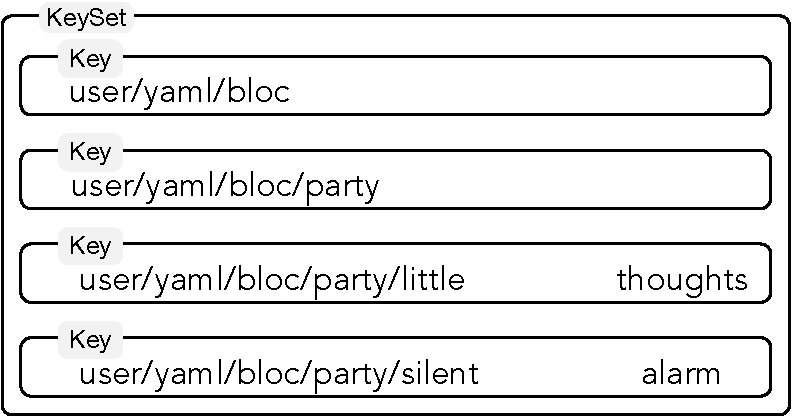
\includegraphics[width=.5\textwidth]{Keys}
  \caption{An exemplary \cc{KeySet}}
  \label{fig:keys}
\end{figure}

For example, the \cc{KeySet} shown in figure~\ref{fig:keys} would then map to the following \glstext{YAML} data, if we use \code{user/yaml} as mountpoint:

\begin{yamlcode}
  bloc:
  bloc/party:
  bloc/party/little: "thoughts"
  bloc/party/silent: "alarm"
\end{yamlcode}

. As we can see the resulting \glstext{YAML} file contains quite a lot of unnecessary redundant data.

In our second solution we take the hierarchical nature of the database into account and split on each part of a key. The result of this approach is the following \glstext{YAML} file:

\begin{yamlcode}
  bloc:
    party:
      little: "thoughts"
      silent: "alarm"
\end{yamlcode}

. The second solution removed unwanted redundancy and reflects the hierarchy much better. However, the approach also has an obvious downside: What happens if we want to store a value in \code{user/yaml/bloc} or \code{user/yaml/bloc/party}? To answer this question, let us look at a tree representing the \glstext{YAML} data from above.

\begin{figure}
  \centering
  \begin{subfigure}[t]{.4\textwidth}
    \centering
    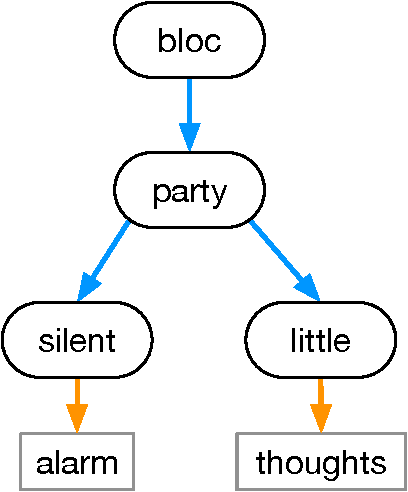
\includegraphics[height=4cm]{Tree}
    \caption{Initial representation}
    \label{fig:tree}
  \end{subfigure}
  \qquad
  \begin{subfigure}[t]{.4\textwidth}
    \centering
    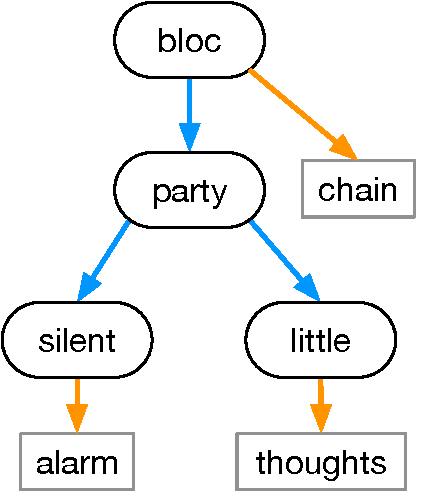
\includegraphics[height=4cm]{TreeExtended}
    \caption{We add an additional value}
    \label{fig:tree_extended}
  \end{subfigure}\\
  \begin{subfigure}[t]{.4\textwidth}
    \centering
    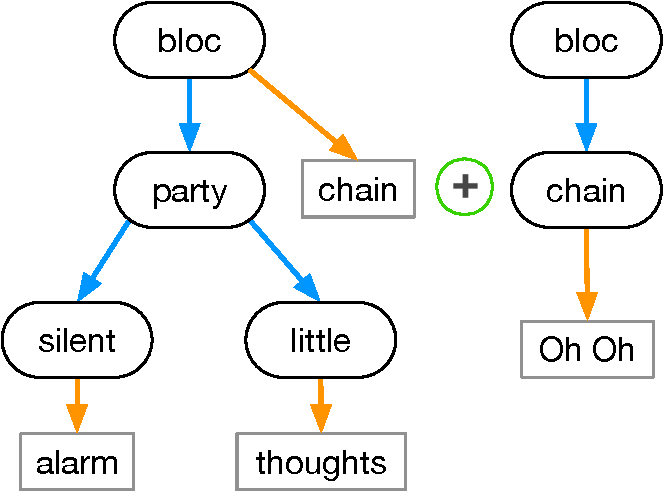
\includegraphics[height=4cm]{TreeExtended+}
    \caption{We add an additional \cc{Key} containing a value}
  \end{subfigure}
  \quad
  \begin{subfigure}[t]{.4\textwidth}
    \centering
    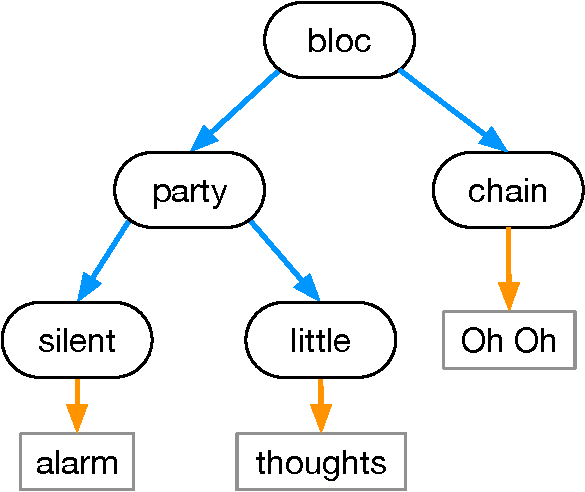
\includegraphics[height=4cm]{TreeExtended++}
    \caption{The new \cc{Key} overwrites the value of the node \code{block}}
    \label{fig:tree_extended++}
  \end{subfigure}
  \caption{The tree-like representation of \glstext{YAML} data shows the problem with adding non-leaf values}
\end{figure}

As we can see in Figure~\ref{fig:tree} the only nodes that store values are the leaves of the tree. Let us assume we also want to store the value \code{chain} in \code{user/yaml/bloc}. Figure~\ref{fig:tree_extended} shows the resulting tree. We could now save \code{chain} as a map key inside \code{bloc}:

\begin{yamlcode}
  bloc:
    chain:
    party:
      little: "thoughts"
      silent: "alarm"
\end{yamlcode}

. However using this approach we are unable to differentiate between the name and the value of a \cc{Key}. For example, if we add a new \cc{Key} with the name \code{user/yaml/bloc/chain} it would just overwrite the value of \code{user/yaml/bloc} (see Figure~\ref{fig:tree_extended++}).

Another option to fix our problem would be to use \glstext{YAML}’s list type, and to store the value of a \cc{Key} and the data below the \cc{Key} as first and second element of the list:

\begin{yamlcode}
  bloc:
    - chain                 # First element stores value
    - party:                # Second element stores data below
      -                     # `user/yaml/bloc/party` contains no value
      - little: "thoughts"
        silent: "alarm"
\end{yamlcode}

. However, this format is quite complicated. If we add support for Elektra’s array type – mapping arrays to \glstext{YAML} sequences – the situation is even worse.

To solve the problem we use another approach. We reserve the name \yaml{___dirdata} to save values in non-leaf nodes. The code below shows the mapping of our example data:

\begin{yamlcode}
  bloc:
    ___dirdata: "chain"
    party:
      little: "thoughts"
      silent: "alarm"
\end{yamlcode}

. Since we reserved the name \yaml{___dirdata} the value below this key will always be a leaf of the tree.

\subsection{Mapping Arrays}

Since Elektra’s array type and \glstext{YAML} sequences are similar, we want to map between these data types.

\begin{figure}
  \centering
    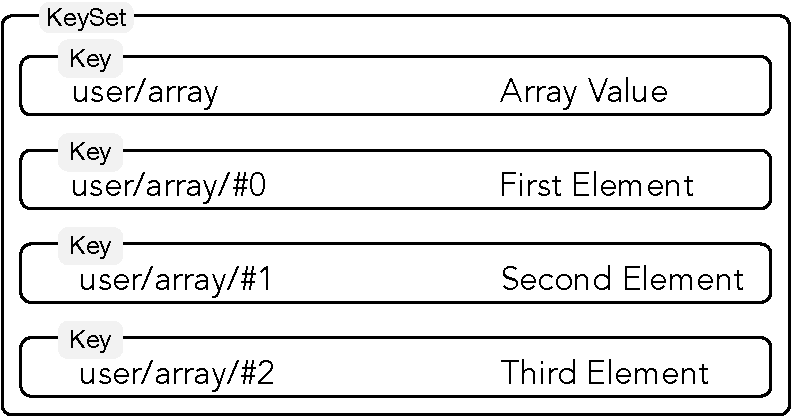
\includegraphics[width=.6\textwidth]{ArrayValue}
  \caption{The \cc{KeySet} above describes an array containing three elements}
  \label{fig:array_value}
\end{figure}

If we use this approach, then the \cc{KeySet} shown in Figure~\ref{fig:array_value} would result in the \glstext{YAML} data:

\begin{yamlcode}
  array:
    - "First Element"
    - "Second Element"
    - "Third Element"
\end{yamlcode}

. We are left with the problem, where to save the data of the \emph{parent} \cc{Key} of the array elements \code{user/array}. We can not use the same approach as before:

\begin{yamlcode}
  array:
    ___dirdata: "Array Value"
    - "First Element"
    - "Second Element"
    - "Third Element"
\end{yamlcode}

, since the result would be a \glstext{YAML} node that is neither list nor map. To fix this problem we decided to convert the \yaml{___dirdata} node to a list element:

\begin{yamlcode}
  array:
    - "___dirdata: Array Value"
    - "First Element"
    - "Second Element"
    - "Third Element"
\end{yamlcode}

. This approach produces valid \glstext{YAML} data and allows us to distinguish between array parents that store values and parents that do not, by checking the first array element for the value prefix \yaml{___dirdata:}.
